\documentclass[9pt,a4paper]{extarticle}
\usepackage[spanish,es-nodecimaldot]{babel}
\usepackage[utf8]{inputenc}
\usepackage[T1]{fontenc}
\usepackage{geometry}
\geometry{margin=1.45cm}
\usepackage{graphicx,float,booktabs,amsmath,caption,hyperref,enumitem}
\setlength{\parindent}{0pt}
\setlength{\parskip}{2.5pt}
\captionsetup{font=small,labelfont=bf}
\setlist{nosep,leftmargin=*,topsep=2pt}
\hypersetup{colorlinks=true,linkcolor=blue,urlcolor=blue}
\title{\vspace{-1.5em}\textbf{Sistema de adquisición y procesamiento de telemetría de vuelo}}
\author{Rodrigo Bravo Bravo\\Ingeniería Aeroespacial -- Primer semestre\\Ruta 1: Telemetría y adquisición de datos}
\date{Noviembre de 2026}
\begin{document}
\maketitle
\vspace{-2em}

\section{Objetivo}
Desarrollar en Python una herramienta de apoyo para una estación terrena que genere un registro simulado de vuelo y procese la telemetría almacenada en CSV. El sistema reproduce una cadena de adquisición y análisis: generación de mediciones, almacenamiento, lectura, validación, filtrado, cálculo de variables derivadas e identificación de eventos. También permite evaluar cómo afecta el ruido de las mediciones al cálculo de la velocidad y cómo cambia el resultado al modificar el tamaño de la ventana. El trabajo se enfoca en el análisis posterior al vuelo de una caja negra, no en el control del vehículo durante su operación.

\section{Metodología y decisiones técnicas}
El simulador genera muestras a 10 Hz (un dato cada 100 ms) y crea \texttt{flight\_log.csv} con las columnas \texttt{time\_ms}, \texttt{altitude\_m}, \texttt{accel\_z\_ms2} y \texttt{temp\_c}. Se representan cinco fases: reposo inicial, propulsión con aceleración neta aproximada de $60\,\mathrm{m/s^2}$, ascenso balístico bajo gravedad, descenso con paracaídas a unos $6\,\mathrm{m/s}$ y reposo final. Se añade ruido gaussiano a la altitud y se insertan tres filas corruptas para probar la robustez del lector. La temperatura disminuye con la altitud usando un gradiente de $0.0065\,^\circ\mathrm{C/m}$.

La aceleración del acelerómetro no equivale siempre a la aceleración cinemática. Con el eje $z$ positivo hacia arriba, en reposo el sensor registra aproximadamente $+9.81\,\mathrm{m/s^2}$ por la fuerza de soporte; durante el vuelo balístico, en caída libre, registra aproximadamente cero. Esta distinción se considera en la simulación. La convención de signos mantiene el eje vertical positivo hacia arriba: durante el ascenso la velocidad es positiva, en el apogeo se aproxima a cero y durante el descenso toma valores negativos. La rapidez media de descenso se reporta como magnitud positiva para facilitar su interpretación.

El procesador lee el CSV fila por fila, comprueba el número de columnas, convierte los campos a números, descarta valores no finitos y exige que el tiempo sea creciente. Después aplica una media móvil centrada de $N=5$ muestras a la altitud. Para cada punto se promedian las mediciones de una ventana alrededor de la muestra actual; cerca de los extremos, la ventana se reduce para mantenerse dentro de los límites del registro. El objetivo es disminuir variaciones rápidas provocadas por el ruido sin eliminar la tendencia general de la trayectoria. Se eligió para el análisis posterior al vuelo: utiliza muestras anteriores y posteriores, por lo que no es causal y no se plantea como filtro para una estación en tiempo real, donde todavía no se conocen las muestras futuras.

La velocidad vertical se estima mediante diferencias finitas. Para los puntos interiores se utiliza la diferencia central:
\begin{equation}
v_i=\frac{h_{i+1}-h_{i-1}}{t_{i+1}-t_{i-1}},
\label{eq:velocidad}
\end{equation}
donde $h$ es la altitud y $t$ el tiempo en segundos. En los extremos se usan diferencias hacia adelante o hacia atrás, porque no existen muestras a ambos lados. La velocidad se calcula tanto con la altitud original como con la filtrada para comparar el efecto del ruido. El despegue se detecta cuando la altitud filtrada supera 5 m; el apogeo es el máximo posterior al despegue; y el aterrizaje se confirma cuando la altitud filtrada permanece en 2 m o menos durante diez muestras consecutivas. Esta última condición evita declarar el aterrizaje por una sola lectura aislada afectada por ruido.

Se utilizó Python y su módulo estándar \texttt{csv} para evitar Pandas y NumPy en los cálculos. Matplotlib se empleó para visualizar las señales y comparar ventanas de filtrado. El programa también genera un segundo CSV con altitud original, altitud filtrada y velocidades estimadas, de modo que los resultados puedan revisarse sin repetir todo el procesamiento. La separación entre generador y procesador permite probar cada etapa de manera independiente y facilita localizar errores.

\newpage
\section{Resultados}
El generador produjo 959 registros válidos y añadió tres registros corruptos. El procesador descartó los tres sin interrumpir la ejecución. Se detectó el despegue a los 2.4 s, el apogeo a los 12.6 s y una altitud máxima de 480.13 m. La velocidad máxima de ascenso estimada fue 87.03 m/s; la rapidez media de descenso, 5.99 m/s; y el tiempo entre los eventos detectados de despegue y aterrizaje, 90.0 s. Los resultados son coherentes con los parámetros usados para construir la simulación: la altitud máxima se encuentra cerca de los 480 m esperados y la rapidez media de descenso se aproxima a los 6 m/s definidos para la fase de paracaídas. La velocidad en las proximidades del apogeo también se mantiene cerca de cero. Los tiempos se obtienen de muestras separadas por 0.1 s y de umbrales seleccionados, por lo que no representan el instante físico continuo exacto.

La Tabla~\ref{tab:ventanas} muestra el efecto del tamaño de ventana. Al aumentar $N$, la velocidad máxima estimada disminuye porque el promedio atenúa variaciones rápidas. En esta simulación, la altitud del apogeo cambia poco, pero una ventana excesiva puede suavizar transiciones reales y alterar la estimación de eventos.
\begin{table}[H]
\centering
\caption{Comparación del tamaño de ventana de la media móvil.}
\label{tab:ventanas}
\begin{tabular}{cccc}
\toprule
$N$ & Apogeo (m) & Tiempo (s) & Velocidad máxima (m/s)\\
\midrule
3  & 480.26 & 12.6 & 88.62\\
5  & 480.13 & 12.6 & 87.03\\
10 & 479.38 & 12.5 & 85.38\\
15 & 478.85 & 12.5 & 83.64\\
\bottomrule
\end{tabular}
\end{table}

En la Figura~\ref{fig:senales} se observa que la derivada de la altitud sin filtrar presenta fluctuaciones más pronunciadas; el suavizado produce una estimación de velocidad más estable. Esto ocurre porque la derivación numérica depende de diferencias entre mediciones cercanas: cuando la altitud contiene ruido, esas variaciones también aparecen en la velocidad y pueden amplificarse. El filtrado previo reduce parte de estas oscilaciones y permite distinguir con mayor claridad el ascenso, el cambio de sentido en el apogeo y el descenso. La Figura~\ref{fig:comparacion} compara las ventanas: las diferencias son pequeñas en altitud, pero más visibles en la velocidad y su máximo. Una ventana corta conserva mejor los cambios rápidos, aunque deja pasar más ruido. Una ventana grande suaviza más la señal, pero puede reducir picos reales y modificar la identificación de eventos. Por ello, el tamaño de ventana representa un compromiso entre estabilidad y conservación de detalles.
\begin{figure}[H]
\centering
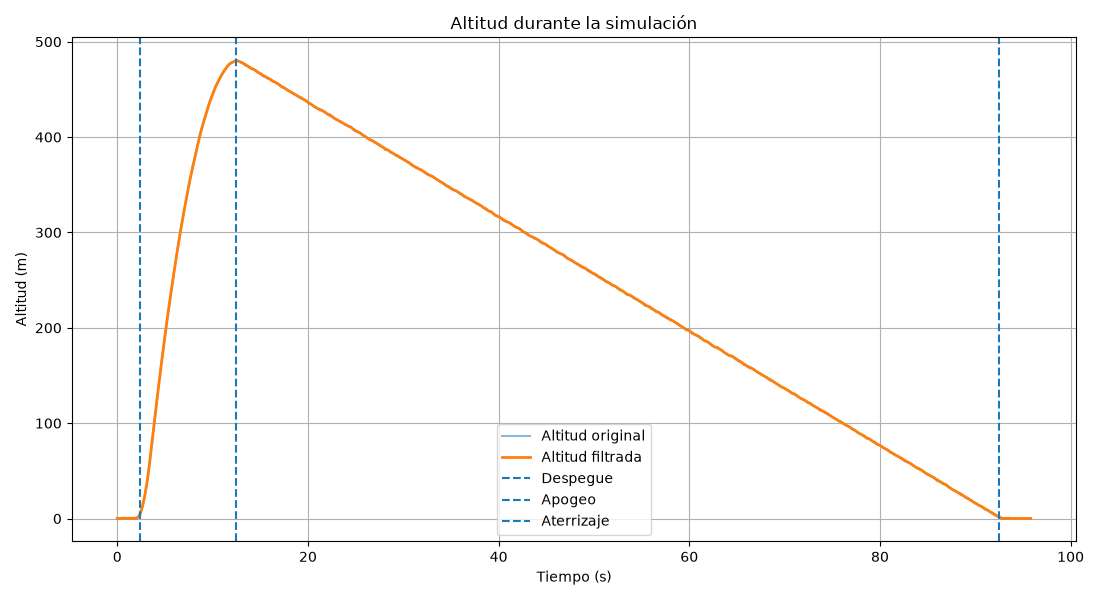
\includegraphics[width=0.48\textwidth,height=3.25cm,keepaspectratio]{../media/plots/altitude_vs_time.png}\hfill
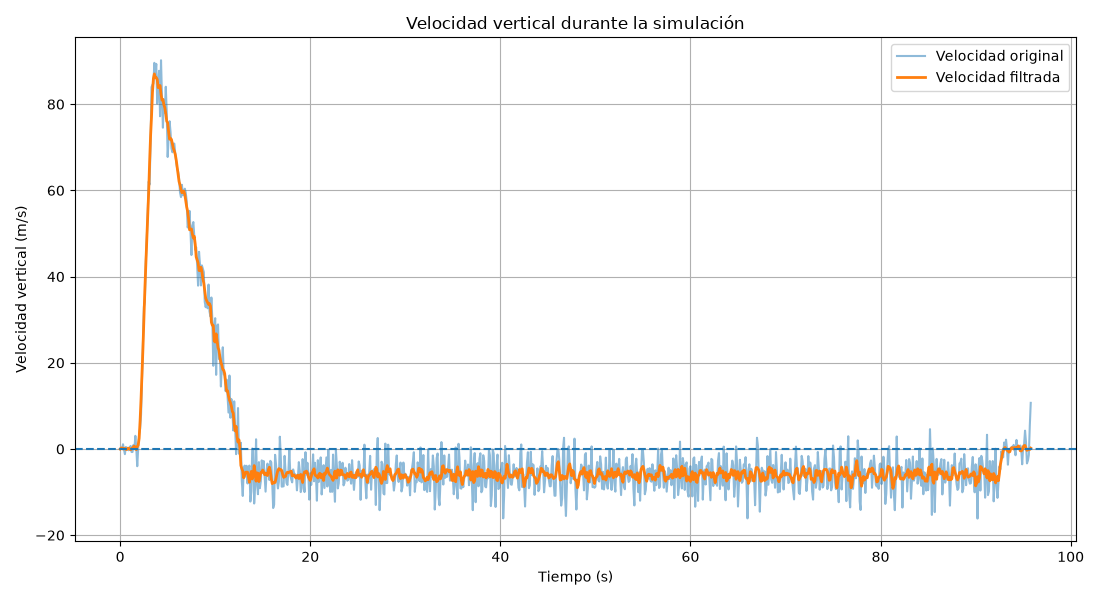
\includegraphics[width=0.48\textwidth,height=3.25cm,keepaspectratio]{../media/plots/velocity_vs_time.png}
\caption{Altitud y velocidad vertical: datos originales y filtrados.}
\label{fig:senales}
\end{figure}
\begin{figure}[H]
\centering
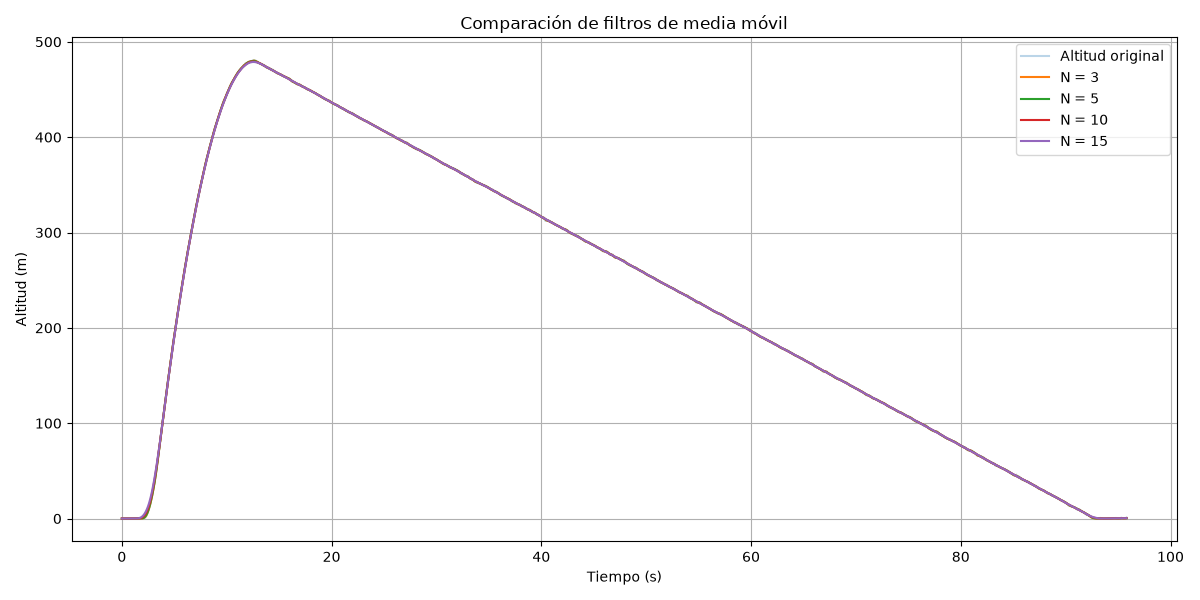
\includegraphics[width=0.48\textwidth,height=3.0cm,keepaspectratio]{../media/plots/comparison_altitude.png}\hfill
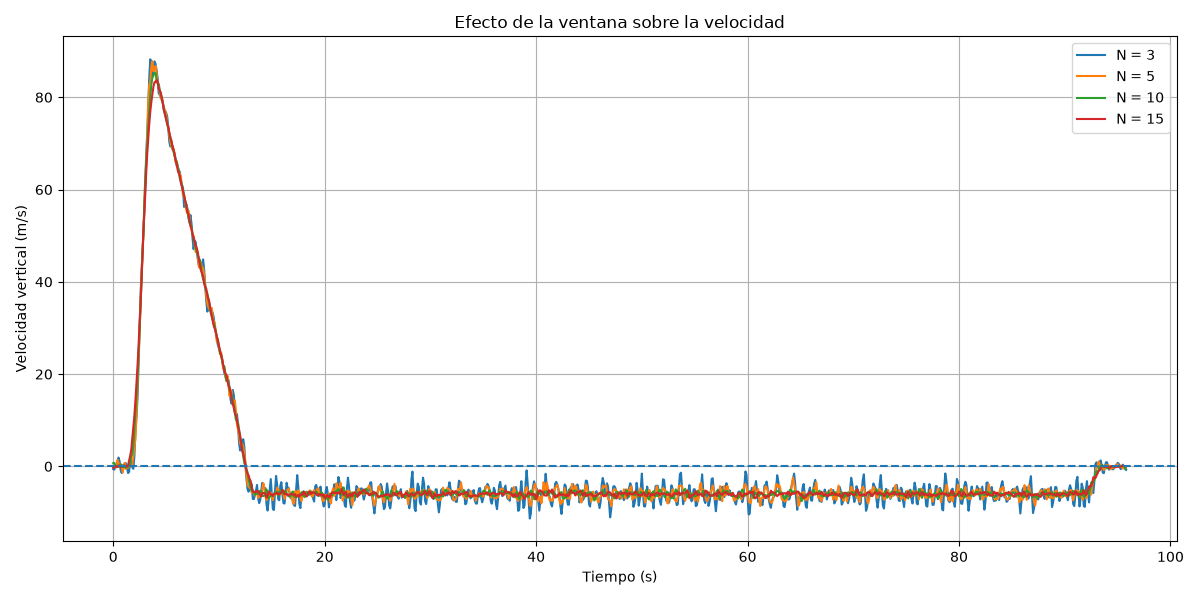
\includegraphics[width=0.48\textwidth,height=3.0cm,keepaspectratio]{../media/plots/comparison_velocity.png}
\caption{Efecto de distintos tamaños de ventana sobre la altitud y la velocidad.}
\label{fig:comparacion}
\end{figure}

\section{Conclusiones}
El programa generó y procesó un registro de vuelo simulado, descartó las tres filas corruptas y calculó métricas para los eventos principales. La separación entre los dos programas permitió distinguir la generación de telemetría de su análisis posterior. Las validaciones evitaron que los registros defectuosos interrumpieran el procesamiento, mientras que el CSV procesado y las gráficas facilitaron la revisión de resultados. La comparación confirmó que el filtrado reduce el ruido de la velocidad, aunque una ventana mayor también atenúa el valor máximo. No basta con elegir la curva más suave: también debe conservar las transiciones y los valores importantes del vuelo. En esta simulación, cinco muestras ofrecen un compromiso razonable para el análisis posterior al vuelo. El resultado es una herramienta inicial de análisis, no una estación terrena completa. Sus limitaciones incluyen el uso de datos simulados, umbrales fijos y una media móvil centrada no causal. Como trabajo futuro se podría implementar un filtro causal, adaptar los umbrales a sensores reales, incorporar recepción en vivo y validar el procesamiento con registros experimentales.

\newpage
\section{Bitácora de trabajo}
El desarrollo se dividió en etapas para probar por separado la generación, lectura, análisis y visualización de la telemetría. Esta organización permitió avanzar de una función básica a la siguiente y comprobar los resultados antes de integrar el flujo completo. También facilitó identificar qué parte debía revisarse cuando una salida no coincidía con lo esperado.
\begin{enumerate}[leftmargin=*,label=\textbf{Etapa \arabic*.}]
\item \textbf{Generación del vuelo.} Se construyó un simulador con muestreo de 10 Hz y cinco fases. Se incorporaron ruido en las mediciones y tres filas corruptas (campo vacío, texto no numérico y columna faltante). La ejecución produjo 959 registros válidos y tres registros intencionalmente inválidos.
\item \textbf{Lectura y limpieza.} Se comprobó que un registro defectuoso no debía detener el procesamiento completo. Se implementaron validaciones del número de columnas, conversión numérica, valores finitos y orden temporal. Las filas que no cumplieron los criterios se omitieron y contabilizaron.
\item \textbf{Cálculo de velocidad.} Al obtener la derivada directamente de la altitud con ruido, la velocidad presentó fluctuaciones amplificadas. Se implementó manualmente una media móvil y se compararon ventanas de 3, 5, 10 y 15 muestras. Se observó que el suavizado mejora la estabilidad, pero reduce la velocidad máxima estimada.
\item \textbf{Detección de eventos.} Se establecieron umbrales para despegue, apogeo y aterrizaje. Para evitar identificar el aterrizaje por una lectura aislada, se exigieron diez muestras consecutivas por debajo del umbral. Los resultados se contrastaron con valores esperados de la simulación: apogeo cercano a 480 m, descenso cercano a 6 m/s y velocidad próxima a cero en el apogeo.
\item \textbf{Generación de resultados.} Se creó un CSV procesado y se generaron gráficas de altitud y velocidad originales y filtradas, además de gráficas comparativas. También se añadieron comprobaciones automáticas para verificar el número de filas descartadas y la coherencia de las métricas principales.
\end{enumerate}

\textbf{Obstáculos, aprendizajes y limitaciones.} La dificultad principal fue controlar el ruido que aparece al derivar numéricamente la altitud. La media móvil redujo las oscilaciones, aunque fue necesario comparar varios tamaños para evitar un suavizado excesivo. También se tuvo que distinguir la aceleración cinemática de la lectura de un acelerómetro en reposo y en caída libre. Finalmente, se identificó que el filtro centrado requiere muestras futuras: es adecuado para procesar la caja negra después del vuelo, pero para una estación terrena en operación sería conveniente sustituirlo por un método causal. Durante la integración también fue necesario revisar la ubicación de los archivos y las rutas relativas de las imágenes para que el documento pudiera compilarse desde la carpeta correcta. Las pruebas de compilación mostraron que la reproducibilidad depende tanto del código como de la organización del proyecto y de las herramientas utilizadas. El trabajo permitió practicar el manejo de CSV, la validación de datos, el cálculo numérico, la visualización con Matplotlib y la documentación técnica de un proceso de adquisición y análisis.

\section{Referencias y uso de herramientas}
\begin{enumerate}[leftmargin=*,nosep]
\item Python Software Foundation. \textit{Python 3 Documentation}. \url{https://docs.python.org/3/}
\item Matplotlib Development Team. \textit{Matplotlib Documentation}. \url{https://matplotlib.org/stable/}
\end{enumerate}
Se utilizó ChatGPT como apoyo para aclarar conceptos, revisar la organización del código y orientar la redacción. La implementación, ejecución y comprobación de los resultados se realizaron en el proyecto.
\end{document}